\footnotesize
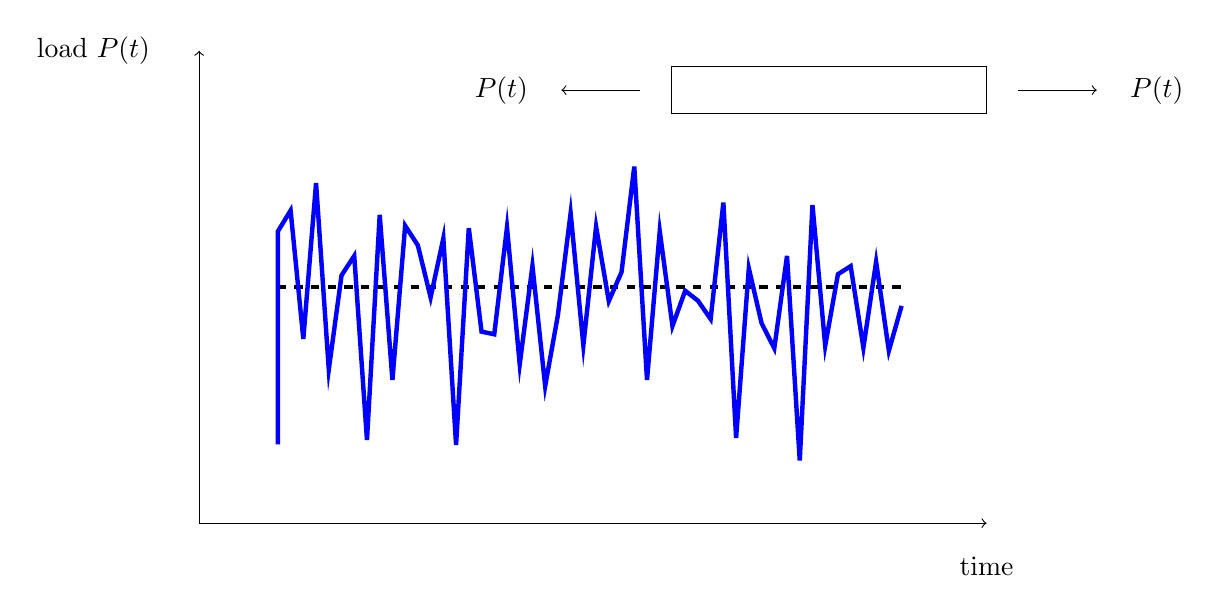
\begin{tikzpicture}[declare function={excitation(\t,\w)=sin(\t*\w);noise=rnd-.5;source(\t)=excitation(\t,20)+noise;filter(\t)=1-abs(sin(mod(\t,50)));speech(\t)=1+source(\t)*filter(\t);}]
\draw[->](0,0)--(10,0)node[below=3mm]{time};
\draw[->](0,0)--(0,6)node[left=5mm]{load $P(t)$};
\draw[dashed,very thick](1,3)--(9,3);
\begin{scope}[xshift=1cm,yshift=1cm]
\draw[blue,ultra thick,x=.022cm,y=2cm](0,0)--plot[domain=0:360,samples=50] (\x,{speech(\x)});
\end{scope}
\begin{scope}[xshift=8cm,yshift=5.5cm]
\draw(-2,-.3)rectangle(2,.3);
\draw[->](2.4,0)--++(1,0)node[right=3mm]{$P(t)$};
\draw[->](-2.4,0)--++(-1,0)node[left=3mm]{$P(t)$};
\end{scope}
\end{tikzpicture}
